\subsection*{Problema 01}

\noindent\textbf{Enunciado:} Calcular la integral:
\begin{align*}
\int -\dfrac{\sqrt[4]{x}}{\sqrt{x}(1 + \sqrt[4]{x})} \, dx
\end{align*}

\noindent\textbf{Solución:} Para resolver esta integral, aplicamos la sustitución sugerida. Sea $u = \sqrt[4]{x}$, de donde se deduce que $x = u^4$ y el diferencial es $dx = 4u^3 \, du$. Además, notamos que $\sqrt{x} = (u^4)^{1/2} = u^2$.

Sustituyendo estas expresiones en la integral original, obtenemos:
\begin{align*}
I &= \int -\dfrac{u}{u^2(1 + u)} (4u^3 \, du)
\end{align*}

Simplificamos la expresión algebraica dentro del integrando dividiendo $u^3$ entre $u^2$:
\begin{align*}
I &= -4 \int \dfrac{u^4}{u^2(1 + u)} \, du \\
I &= -4 \int \dfrac{u^2}{1 + u} \, du
\end{align*}

Como el grado del numerador es mayor que el del denominador, realizamos la división polinómica o un ajuste algebraico sumando y restando $1$ en el numerador:
\begin{align*}
\dfrac{u^2}{1 + u} &= \dfrac{u^2 - 1 + 1}{1 + u} \\
&= \dfrac{(u - 1)(u + 1)}{1 + u} + \dfrac{1}{1 + u} \\
&= u - 1 + \dfrac{1}{1 + u}
\end{align*}

Reemplazamos esto en nuestra integral:
\begin{align*}
I &= -4 \int \left( u - 1 + \dfrac{1}{1 + u} \right) du
\end{align*}

Integramos término a término:
\begin{align*}
I &= -4 \left( \dfrac{u^2}{2} - u + \ln|1 + u| \right) + C \\
I &= -2u^2 + 4u - 4\ln|1 + u| + C
\end{align*}

Finalmente, regresamos a la variable original $x$ sustituyendo $u = \sqrt[4]{x}$:
\begin{align*}
I &= -2(\sqrt[4]{x})^2 + 4\sqrt[4]{x} \\
&\quad - 4\ln|1 + \sqrt[4]{x}| + C \\
I &= -2\sqrt{x} + 4\sqrt[4]{x} \\
&\quad - 4\ln|1 + \sqrt[4]{x}| + C
\end{align*}

\begin{figure}[H]
	\centering
	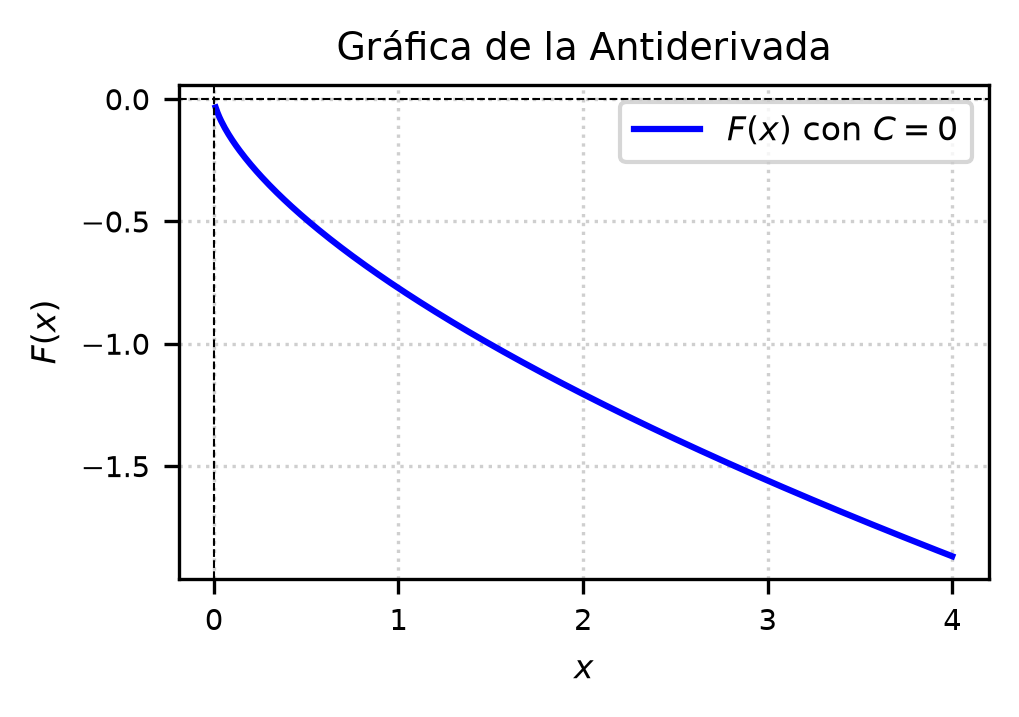
\includegraphics[width=\columnwidth]{semana_05/graficas/SEM05_P01_grafica.png}
	\caption{Representación gráfica de $f(x)$ y su antiderivada $F(x)$ evaluada para la constante de integración $C = 0$ (Problema 01).}
	\label{fig:problema01}
\end{figure}
